\documentclass[12pt, letterpaper]{article}


% Include supporting packages
\usepackage[top=1in, bottom=1in]{geometry}
\usepackage{setspace}
\usepackage{amsmath}
\usepackage{enumitem}
\usepackage{setspace}
\usepackage{url}
\usepackage{graphicx}
%\usepackage{cite}
%\usepackage{hyperref}


% Set double spacing
%\doublespacing

% Formatting for Title, starting halfway down the first page
\usepackage{titlesec}
\titleformat{\section}{\normalfont\Large\bfseries}{}{0em}{}


\setlength\headheight{24pt}
\usepackage{fancyhdr}
\pagestyle{fancy}
\fancyhf{}
%\fancyhead[R]{Author Last Name: Shortened Title}
\fancyfoot[C]{\thepage}

\begin{document}

\vspace*{.5in} % Pushes the title  down page 1
\begin{center}
    {\LARGE \bfseries Pocket FT8 Transceiver Revisited} \par
    \vspace{0.25in}
    {\large Jim Conrad, KQ7B} \par
    {132 Mill Creek MDW, Grangeville, ID 83530 USA}
\end{center}

\begin{center}
The Pocket FT8 Transceiver Revisited is a self-contained, portable software defined QRPP transceiver.
\end{center}

\section{Introduction and Features}

Charles Hill's original Pocket FT8 project\cite{pocketFT8} inspired several fully self-contained FT8 transceiver derivatives\cite{dxFT8}\cite{tinyDX} in which the computer \textit{is} the radio.
This derivative revisits the original concept with simplified hardware and enhanced firmware while retaining the pocket-size, single-band, QRPP, HF transceiver concept for outdoor adventuring. 
Features include:
  \begin{itemize} [noitemsep]
  \item Open source hardware and firmware
  \item Self-contained and light-weight
  \item Compact, 4-layer PCB (4.0X2.8")
  \item FSK FT8 modulator/demodulator
  \item 275+ mW RF output (QRPP)
  \item RF filter slot
  \item Low jitter TCXO
  \item GPS disciplined date, time and location (grid square)
  \item 480x320 pixel TFT calibrated touchscreen
  \item Waterfall traffic display
  \item Standard FT8 QSO sequencer
  \item Automatic QSO logging to an  ADIF file
  \item JSON station configuration file
  \item Operation from a  5V USB power bank
  \end{itemize}
The FT8 protocol\cite{qexFT8}, designed for weak signal communication is ideal for portable, battery-operated, QRPP operation.
While traditional  setups consist of a  computer, transceiver, and, in some cases, an audio interface,  Pocket FT8  integrates these  functions in a single, self-contained package.
The use of FT8 reduces the transceiver's power requirements and weight while also  eliminating the telegraph key, microphone, and headset accessories accompanying SSB/CW transceivers.
Consolidating the  radio with the FT8 encoder/decoder in an embedded computer eliminates the need to pack a computer in  addition to the radio.
Further integration of a GPS receiver provides the UTC date and time for ADIF logging as well as the Maidenhead grid square and FT8 time-synchronization.
Of course, FT8 QSOs are  terse, contest-like exchanges conveying sequenced,  structured messages with minimal operator intervention after contact has been established.
Although FT8 is not always appropriate, commercial alternative designs\cite{kh1}\cite{qmx}  cover many of those situations.

\section{CONFIG.JSON}
The radio requires an SD card in the Teensy card slot containing a station configuration file entitled, CONFIG.JSON.
A sample JSON configuration file appears in Figure \ref{fig:config}.

Only two parameter entries, the station's callsign and operating frequency, are required; all remaining parameters illustrated in Figure \ref{fig:config} may be omitted.
The callsign must conform to the WSJTX requirements.
The operating frequency must be provided in kHz (without a fraction) and it must be compatible with the low-pass filter installed in the filter slot, FL1.

The operator's personal name is optional and is included in log file entries when provided.

The optional M0, M1 and M2 entries program three possible ``canned" 13-character FT8 ``free text" messages.

When GPS is not reliable, the station's 4-character maidenhead grid square locator may be configured manually.

The Si4735 automatic volume control feature may optionally configured off (false) or on (true). 
The default is on (true).

The FT8 QSO sequencer, affectionately (satirically?) known as ``RoboOp,"  retransmits this station's last message when it receives no or an unexpected response from the remote station until the qsoTimeout period (in seconds) expires.
By default, RoboOp tracks recently worked stations and avoids contacting duplicates; the enableDuplicates parameter will override this prohibition.

Successful QSOs, those exchanging callsigns and signal reports, are logged to an ADIF file whose name may be optionally configured to override the default, ``LOGFILE.ADIF".
The log file is always written to the Teensy SD card.
If your station is located at a SOTA site, you may wish in configure a SOTA Reference Number to be included in the log file.

\section{Operation}
The only truly required connections to the radio are power, antenna and the SD card containing the CONFIG.JSON file.
Five volt power is supplied through the Teensy 4.1's USB Micro-B port.
The antenna must be connected to the transceiver's SMA port.
The SD card must be inserted in the Teensy slot, not the unsupported Adafruit display slot.

The use of a connected GPS improves the transceiver's usability and is strongly recommended.
The GPS connection is made with a 5-pin ribbon cable to J3.
A GPS fix automatically configures the station's maidenhead grid square locator as well as the UTC date and time.
Without the GPS, the transmitter will use the manually configured locator, and will restore the date and time from Teensy's battery-backed clock.
Without the GPS, the station's timezone is unknown and QSOs may not be logged using UTC time as required by ADIF.
Without the GPS, the transceiver's knowledge of the FT8 15-second timeslot boundaries drifts with the battery-backed clock.
Use the GPS whenever possible.


  
 \section{Hardware Overview}
The Pocket FT8  transceiver (Figure \ref{fig:schematic}) is designed around a Teensy 4.1, 600 mHz, 32-bit ARM Cortex-M7 MCU with hardware floating point, USB, SPI, I2C, 1 mB of RAM, and two ADCs.

When transmitting, the MCU reprograms the Si5351 clock generator's output for each of the eight FT8 Frequency Shift Keying (FSK) tones, a direct FSK scheme, unlike the Audio FSK (AFSK) widely used with a SSB transmitters' microphone jack.
Frequency stability is achieved by locking the Si5351 to a low jitter Temperature Controlled Crystal Oscillator (TCXO) reference.
The Si5351's output is buffered by one element of a SN74ACT244 octal bus driver whose remaining seven buffers function in parallel as the transmitter's QRPP power amplifier (PA).
A five-pole Chebyshev low-pass filter  with 1 dB of ripple (Figure \ref{fig:lpFilter}) peaking near the expected operating frequency  provides harmonic rejection.
The PA delivers 275 mW through the filter.

An Si4735 digital receiver implements the receiver's RF section and delivers FT8 audio tones to the Teensy audio pipeline via ADC2.
While the Si4735  lacks the performance of alternative designs, its capabilities are on par with the QRPP transmitter:  on-the-air experience found the receiver decodes more signals than the 275 mW transmitter can work, especially in crowded band conditions.
The development of an early prototype found the Si4735 performance degrades in the presence of noise from other I2C bus device traffic; the problem was resolved by isolating the Si4735 on a private I2C bus.
The Si4735's phase-locked loop (PLL) locks to the Si5351 clock generator's CLK2 output.

An Adafruit 3.5" TFT 320x480 touchscreen with an HX8357D controller serves as the graphical user interface device.
The display achieves satisfactory performance over an SPI bus from the MCU while the resistive touchscreen connects to the MCU's ADC1.
The compact display is ideal for portable operation,  but touchscreen accuracy improves with use of a stylus rather than your finger.








 
 \subsection*{FL1 Design}
FL1 mainly provides harmonic rejection for the transmitted signal.
On 40 meters, the five pole Chebyshev design provides for 1 dB of ripple peaking inside the band.

During receive, the Chebyshev low-pass design offers only minimal rejection of out-of-band signals. 
While this has not proven to be a significant issue in the wilderness use-case, the receiver might benefit from a bandpass design in other applications.
 \subsection*{Hardware Construction}

\subsection*{T1}
T1 is a broadband, bifilar wound transformer consisting of 10 turns of 26 AWG on an FT37-43 core.

\subsection*{FL1}
The FL1 low-pass filter can be assembled and tested on a small daughter board.
With some effort, it can probably be made pluggable to facilitate band changes.

\section{Software}
\subsection*{Software Design}

\subsection*{Software Construction}


\section{Testing}

\section{Operation}

\section{Future}

\section{Acknowledgements}


% Schematic
\begin{figure}[b]
\centering
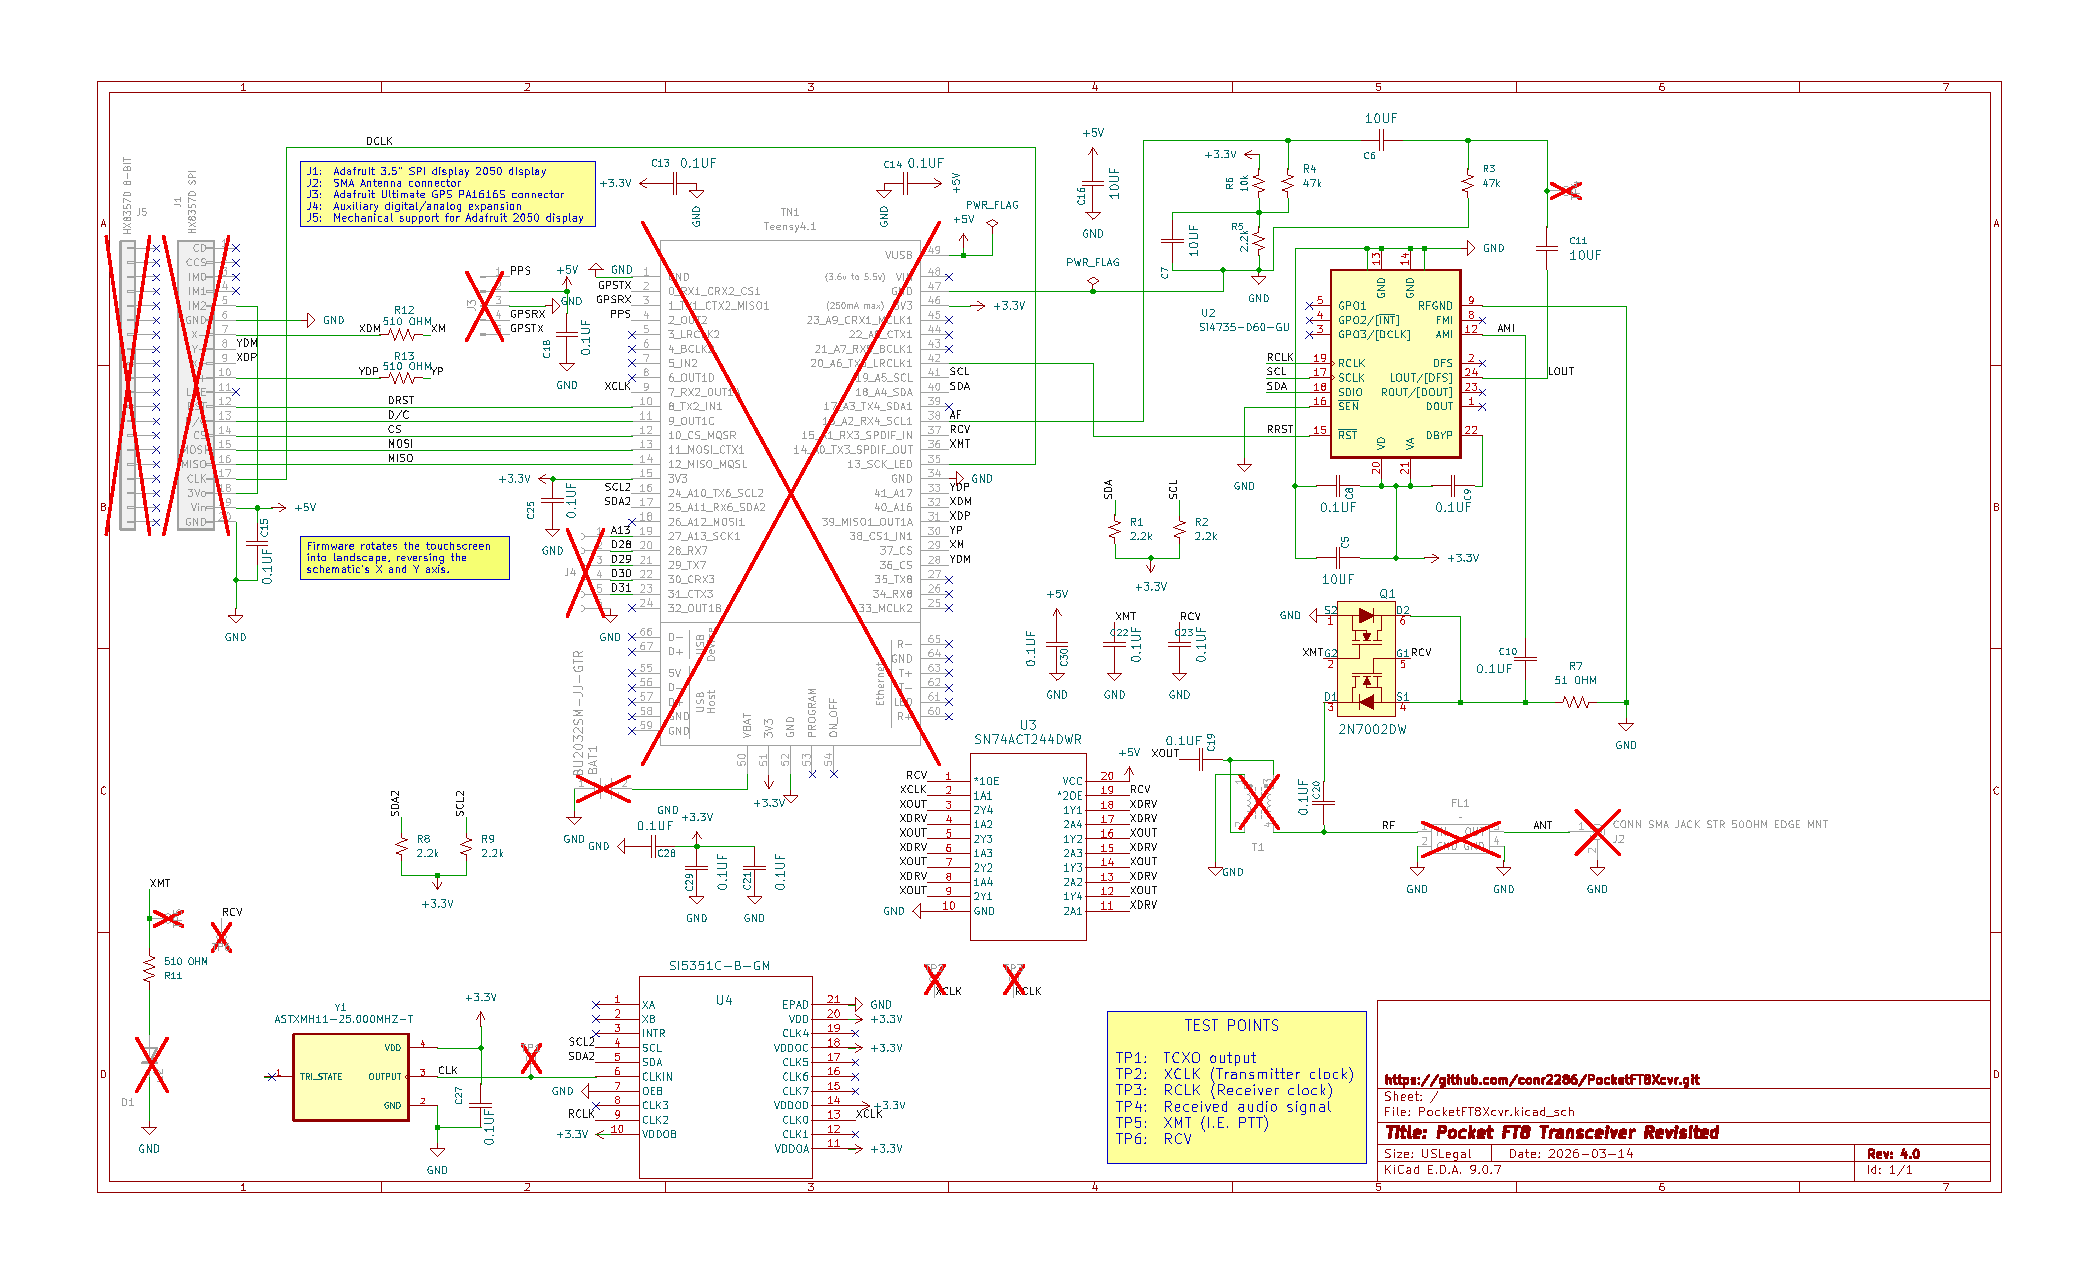
\includegraphics[width=0.9\textheight, angle=90]{images/Schematic.pdf}
\caption{Schematic}
\label{fig:schematic}
\end{figure}

% Chebyshev Low-Pass Filter Bode Plot
\begin{figure}[b]
\centering
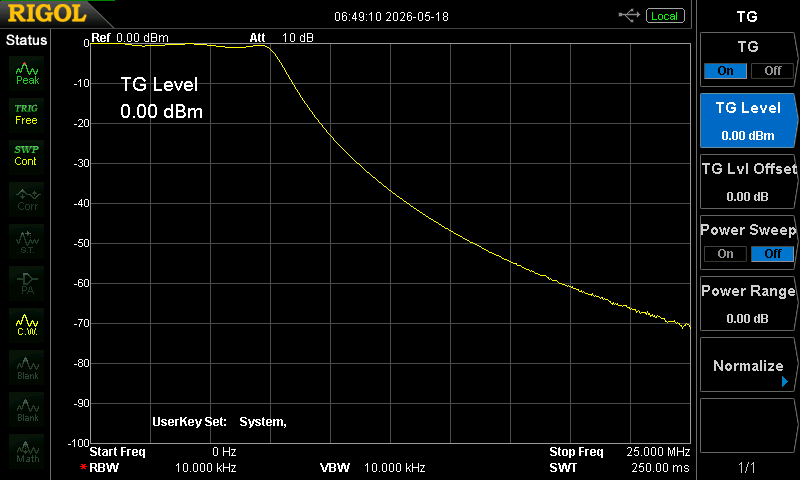
\includegraphics[width=1.0\textwidth]{images/LPfilter.png}
\caption{Chebyshev Low-Pass Filter Bode Plot}
\label{fig:lpFilter}
\end{figure}

% CONFIG.JSON
\begin{figure}[htbp]
\centering
\begin{verbatim}
//-CONFIG.JSON-------------------------------------------------------------
{
   "callsign": "W1AW",              //REQUIRED:  Station callsign
   "frequency": 7074,               //REQUIRED:  Operating frequency in kHz
   "myName" : "Jim",                //OPTIONAL:  Operator's personal name
   "M0" : "CQ KQ7B/IDAHO",          //OPTIONAL:  13-Char Free Text Msg0
   "M1" : "IDAHO",                  //OPTIONAL:  13-Char Free Text Msg1
   "M2" : "QRT"                     //OPTIONAL:  13-Char Free Text Msg2
   "tcxoCorrection": -5,            //OPTIONAL:  TCXO freq correction in Hz
   "locator": "",                   //OPTIONAL:  4-char maidenhead grid
   "enableAVC": true,               //OPTIONAL:  0=disabled, 1=enabled
   "qsoTimeout": 180,               //OPTIONAL:  Seconds RoboOp will retry
   "enableDuplicates": false,       //OPTIONAL:  Enable duplicate contacts
   "logFilename" : "LOG0815.ADIF",  //OPTIONAL:  ADIF logfile name
   "my_sota_ref" : "W7I/IC-257",    //OPTIONAL:  SOTA Reference Number 
}
\end{verbatim}
\caption{CONFIG.JSON}
\label{fig:config}
\end{figure}


%\newpage
\bibliographystyle{IEEEtran}
%\bibliographystyle{plain}
%\bibliographystyle{ieeetr}
\bibliography{PocketFT8Revisited}
\end{document}


